\documentclass[conference]{IEEEtran}
\usepackage{graphicx,cite,url}
\renewcommand{\ttdefault}{lmtt}
\pdfinfo{/Author (RISC-V CPU) /Creator () /Producer () /Title (5-Stage Pipelined RISC-V Processor)}
\title{5-Stage Pipelined RISC-V Processor}
\author{\IEEEauthorblockN{Aryan Kinha, Preetish Ubhrani, Divyanshu Singh,\\Jatin Kumar Singh, Jatin Verma}
\IEEEauthorblockA{Newton School of Technology, Rishihood University}}
\begin{document}
\raggedbottom
\maketitle
\begin{abstract}
The Phase I processor executes a small RISC-V instruction subset through five pipeline stages. The Verilog implementation keeps each instruction's data and control signals together as it moves from fetch to write-back. Separate instruction and data memories allow fetch and load/store access in the same cycle. Branches are resolved in EX, where a taken branch clears the younger instructions. Programs use NOPs to separate data dependencies because this version has no hardware interlock. A write-through register file lets ID read a result during the producer's WB cycle. Verification covers individual modules, final register and memory states, and simultaneous stage occupancy. All supplied tests pass. The cycle and retirement counts record when each test finishes; a performance comparison is reserved for Phase II. The supported subset and memory restrictions are stated explicitly so that the prototype's limits can be checked alongside its behavior.
\end{abstract}
\begin{IEEEkeywords}
RISC-V, Verilog, processor pipeline, instruction decoding, functional simulation
\end{IEEEkeywords}

\section{Literature Review}
\subsection{Instruction set and implementation choices}
The RISC-V unprivileged specification defines instruction encodings and their effects on registers, memory and control flow~\cite{isa}. Implementations can choose different datapaths while preserving those effects. Our processor implements only the selected arithmetic, memory and branch operations. It does not cover the complete RV32I base ISA or provide architectural traps. This small subset lets us trace useful programs through the pipeline without adding execution units that Phase I does not need.

Patterson and Hennessy describe how processor datapaths and control determine instruction execution~\cite{patterson}. A single-cycle processor completes an instruction's required operations between active clock edges. Its longest supported path sets the clock period, even when another instruction needs less work. A multi-cycle processor divides execution into steps and can reuse hardware. Its controller must select those steps and retain intermediate values. Both organizations help explain the tradeoffs behind the pipeline used here; neither is implemented as a baseline in Phase I.

Harris and Harris develop RISC-V processors from digital logic, covering single-cycle, multi-cycle and pipelined designs~\cite{harris}. Pipeline registers let different instructions occupy different stages at once. They also add state: every saved operand must remain paired with the right instruction and control bits. The steps within one instruction still occur in order. Our tests therefore check stage movement as well as the final register and memory values.

\subsection{Hazards and usual remedies}
A structural hazard occurs when instructions need the same hardware resource at the same time. Separate instruction and data memories remove the conflict between fetching an instruction and accessing data. Both memories have combinational read paths. They provide fixed stage timing in this prototype; caches and variable-latency external memory are outside its scope.

A read-after-write hazard occurs when a consumer reads a register before its producer makes the new value available. Forwarding supplies a later stage's result directly to the consumer. A load-use interlock stalls when the required load value is still unavailable. Software can also schedule independent instructions or NOPs between dependent operations. Phase I uses this scheduling approach. Every supplied program must follow the padding rule because the processor cannot stall an incorrectly scheduled consumer.

Write-after-read and write-after-write hazards can arise when operand reads or writes occur out of order. Here, instructions advance in order, read operands in ID and write registers in WB, with no variable execution latency. These ordering hazards need no separate handling. Branches create a different problem: fetch continues before the branch decision is known. Earlier resolution, prediction and fetch stalls are common approaches~\cite{patterson,harris}. Our processor fetches sequentially until EX redirects the PC, then discards the younger instructions.

\subsection{Small public RISC-V cores}
PicoRV32 is a compact core with options for its register file, memory interface and instruction support~\cite{pico}. Its documentation gives a useful example of a small core with a clearly defined memory interface. Ibex is a configurable SystemVerilog core with a broader feature set and an extensive verification effort~\cite{ibex}. Those projects go beyond the current prototype. For Phase I, we specify a fixed subset and test its behavior directly.

VexRiscv uses SpinalHDL and supports configurable pipeline stages, bypass paths and interlocks~\cite{vex}. Its operand-routing and hazard options provide a comparison for the fixed EX operand selection used here. Our design has no plugin system or configurable hazard hardware. CORE-V CV32E40P is an in-order pipelined core with a wider instruction scope and a separate verification project~\cite{cv}. These cores illustrate different choices for stage boundaries and interfaces. We consulted their documentation for comparison and wrote the RTL for this project's Phase I requirements.

The student repository \texttt{risc-5-processor} checks its CPUs with an instruction model, directed edge cases and repeatable random programs~\cite{comparison}. We used those verification ideas to extend this prototype's tests. Our checker is written for the selected instruction subset and its NOP scheduling rule.

\section{Proposed Solution}
\subsection{Datapath and scope}
The processor has IF, ID, EX, MEM and WB stages, separated by IF/ID, ID/EX, EX/MEM and MEM/WB registers. Fig.~\ref{fig:block} shows the datapath, the write-back connection and EX branch redirection. All state changes on the rising edge of one clock. The synchronous active-high reset clears the PC, writable machine state and pipeline valid bits. Instruction memory loads the selected hex file with \texttt{\$readmemh}; reset leaves the program intact.

\begin{figure*}[t]
\centering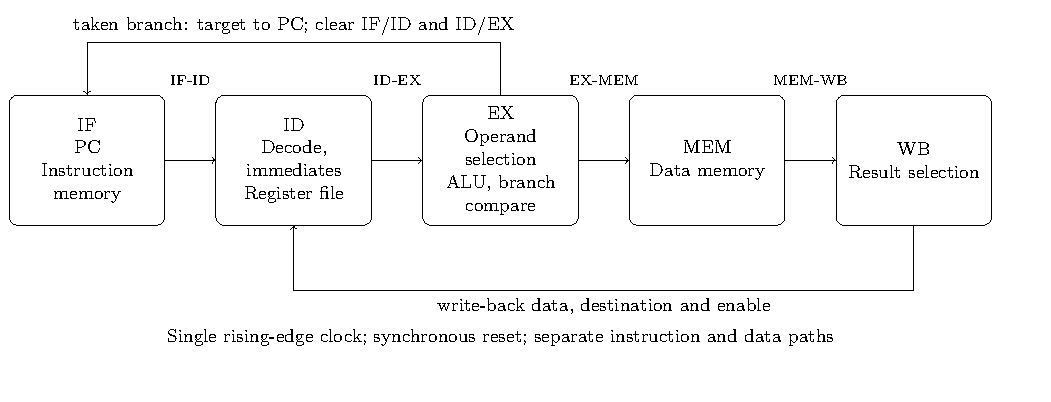
\includegraphics[width=\textwidth]{../diagrams/block.pdf}
\caption{Pipeline stages and registers, with separate memories, the write-back connection and EX branch redirection.}
\label{fig:block}
\end{figure*}

\begin{figure*}[t]
\centering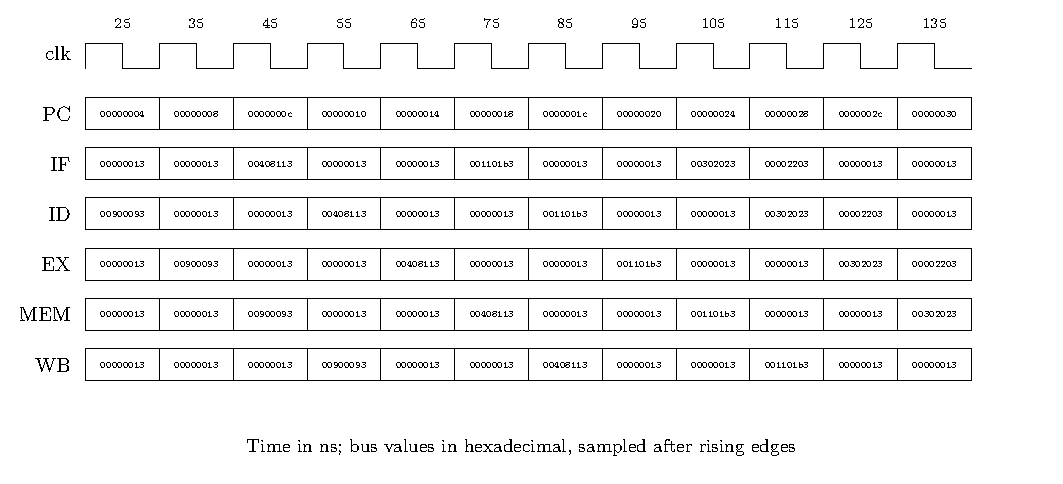
\includegraphics[width=\textwidth]{../waveforms/dependencies.pdf}
\caption{Dependency-program VCD showing the clock, PC and stage instruction words. Hexadecimal bus values are sampled just after rising edges. The NOP word is 00000013; the valid bits distinguish executed NOPs from bubbles.}
\label{fig:wave}
\end{figure*}

The register file stores word-sized values. Reads of x0 return zero, and writes to x0 are ignored. Each memory holds 64 words. The arrays use word indices, but the PC, effective addresses and branch offsets use standard byte addresses. An aligned address selects a word with its low alignment bits set to zero. Sequential execution advances the PC by four bytes.

The memory wrapper supports aligned addresses within the local storage range. An invalid or misaligned instruction fetch returns NOP. An invalid data read returns zero, and an invalid data write has no effect. These rules keep array accesses defined without adding access-fault or misalignment traps. The saved demonstration programs use valid local addresses; verification-only edge cases also check invalid data accesses. The design has no interrupts, caches or bus handshakes.

\subsection{Instructions and decoding}
The accepted encodings are listed in Table~\ref{tab:enc}. ADD and SUB use the R format. ADDI and LW use an I immediate, while SW reconstructs the split S immediate. Branch decoding reconstructs the B immediate, including its implicit low zero bit. Immediates are sign-extended before arithmetic. ADD and SUB wrap at the register width. LW and SW access whole words. BEQ tests equality and BNE tests inequality. NOP uses the standard ADDI encoding with zero source, destination and immediate.

\begin{table}[t]
\caption{Accepted encoding fields, written in hexadecimal}
\label{tab:enc}\centering
\begin{tabular}{lccc}\hline
Instruction & Opcode & funct3 & funct7\\\hline
ADD & 33 & 0 & 00\\
SUB & 33 & 0 & 20\\
ADDI & 13 & 0 & --\\
LW & 03 & 2 & --\\
SW & 23 & 2 & --\\
BEQ & 63 & 0 & --\\
BNE & 63 & 1 & --\\\hline
\end{tabular}
\end{table}

The decoder checks the required operation fields as well as the opcode. Unsupported encodings leave side-effect controls low and clear the supported signal. ID combines this signal with the incoming valid bit. An unsupported entry can pass through the registers, but it cannot change machine state or retire. The prototype does not raise an illegal-instruction exception.

Table~\ref{tab:ctrl} lists the decoded control bits. The load control selects memory data in WB, so the design needs no extra write-back select bit. Branch comparison uses the original register values, independently of the ALU result. Each control bit travels with the instruction's data.

\begin{table}[t]
\caption{Control values for supported instructions}
\label{tab:ctrl}\centering\small
\begin{tabular}{lccccccc}\hline
 & RW & MR & MW & Imm & Sub & Br & NE\\\hline
ADD  &1&0&0&0&0&0&0\\
SUB  &1&0&0&0&1&0&0\\
ADDI &1&0&0&1&0&0&0\\
LW   &1&1&0&1&0&0&0\\
SW   &0&0&1&1&0&0&0\\
BEQ  &0&0&0&0&0&1&0\\
BNE  &0&0&0&0&0&1&1\\\hline
\end{tabular}
\par\smallskip\footnotesize RW: register write; MR/MW: memory read/write; Imm: immediate ALU operand; Sub: subtraction; Br: branch; NE: inequality.
\end{table}

\subsection{Pipeline state and stage operation}
IF reads the instruction at the current PC. At the active edge, IF/ID captures the word and its address. ID extracts register numbers, reads the register file and decodes the immediate and controls. ID/EX saves these values for EX. Execute selects the ALU operands, calculates the result and adds the branch immediate to the branch instruction's saved PC.

EX/MEM stores the arithmetic result or effective address, the original store operand and the controls needed downstream. MEM accesses data storage only when a valid entry enables the corresponding read or write. MEM/WB holds the ALU result and load value. WB selects the load value for LW and the ALU result for other register-writing instructions. Its write enable also requires a valid entry.

Source and destination register numbers remain available in ID/EX, EX/MEM and MEM/WB for later dependence checks. Phase I carries these fields without using them to detect hazards. The registers also hold the instruction word, its PC and a valid bit. Clearing validity and the side-effect controls creates a bubble. A bubble displays the NOP encoding, so the valid bit distinguishes it from a NOP that actually executes.

Fig.~\ref{fig:pipe} shows the stage sequence. The simulation checks overlap from the stage-valid signals and instruction addresses. Two NOPs at different PCs are separate instructions even though their words match.

\begin{figure}[t]
\centering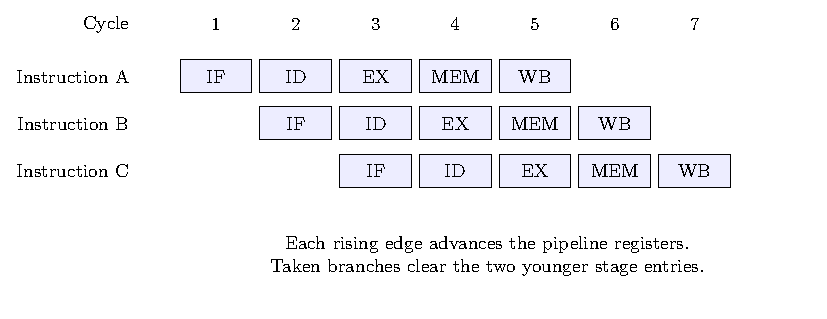
\includegraphics[width=\columnwidth]{../diagrams/pipeline.pdf}
\caption{Stage sequence for successive instructions without a branch redirect. This sketch shows the timing convention.}
\label{fig:pipe}
\end{figure}

\subsection{Branch handling}
EX adds the signed branch immediate to the saved PC to calculate the target. If a valid BEQ or BNE meets its condition, the next edge loads that target into the PC and clears IF/ID and ID/EX. The branch itself advances to EX/MEM. The instruction in ID and the sequential instruction in IF are discarded before they can change state. Older instructions continue through the pipeline.

A taken branch costs two younger instruction slots. There is no delay slot. A not-taken branch leaves both pipeline registers intact. The branch program tests forward targets, a backward loop and both outcomes of BEQ and BNE. Discarded paths contain register writes and stores, so a missing flush changes the expected final state.

\subsection{Data-dependence scheduling}
The register file writes on the rising edge and reads combinationally. If WB writes the same nonzero register that ID is reading, the read port returns the current write data. This write-through path stays inside the register file. There is no EX/MEM-to-EX forwarding path or hazard detector.

A writer and its first dependent reader need two intervening instructions. With that spacing, the writer is in WB while the reader is in ID. At the next edge, ID/EX captures the value supplied by register-file write-through. One intervening instruction would make the reader capture its operands too early. Loads follow the same rule: their data is already in MEM/WB during WB.

The dependency program uses exactly two NOPs at each such boundary. Independent instructions can fill the same slots. The rule covers every register operand, including branch comparisons, store addresses and store data. A store followed by a load from the same address needs no padding for the memory access itself, because the store reaches MEM first. The load still needs padding if a recent register write supplies its address. Incorrectly scheduled dependencies produce stale operands; the hardware does not repair them.

\subsection{Prototype verification status}
The runner compiles and simulates the tests with Icarus Verilog~\cite{icarus}. The ALU bench checks addition, subtraction and wraparound. Register-file tests cover reset, saved writes, x0 and write-through on both read ports. Control tests exercise every supported operation, nearby unsupported encodings and signed immediate reconstruction. GNU RISC-V binutils assembled the four saved assembly programs, and the emitted words matched the checked encodings. Each program runs in a fresh simulation. The top-level bench compares every register and data-memory word with its expected-state file.

A separate Python instruction model checks the saved expected-state files and every RTL retirement's PC, instruction word and register write. Before these comparisons, it passes 8 hand-calculated model cases and 4 fixed encoding checks. The extended suite passes 19 RTL program runs: the original 4, 3 directed edge cases and 12 repeatable random cases. The added cases exercise repeated destinations, x0, memory overwrite and boundary behavior, invalid data addresses and branch shadows. Random cases retain the two-NOP padding rule and use forward branches to guarantee termination. Test images and expected states for these runs remain in the build directory.

The bench also writes a CSV trace with stage PCs, valid bits, WB effects and the taken-branch signal, sampled before each active edge. Every run checks that cycles equal retired instructions plus pipeline fill and the taken-branch flush cost. This accounts for the observed timing without introducing a baseline or a performance study.

An instruction retires when a valid supported entry reaches its WB completion edge. This includes NOPs, stores and branches, even when they write no register. Flushed entries do not retire. A store changes memory in MEM, before it reaches WB. The cycle counter starts at the first rising edge after reset release and stops when the program's final instruction completes WB. The testbench defines this stopping point; the CPU has no halt instruction.



All directed tests pass: 8 ALU cases, 37 register-file cases and 14 control cases. Table~\ref{tab:runs} records the program completion counts, including software padding and pipeline fill. Phase I makes no clock-frequency, speed-up or CPI claim.

\begin{table}[t]
\caption{Functional program runs}
\label{tab:runs}\centering
\begin{tabular}{lrr}\hline
Program & Cycles & Retired\\\hline
Arithmetic & 13 & 9\\
Load/store & 14 & 10\\
Branches and loop & 41 & 29\\
Padded dependencies & 21 & 17\\\hline
\end{tabular}
\end{table}

Fig.~\ref{fig:wave} plots the dependency program's VCD. The instruction words advance across the stage boundaries, separated by the scheduled NOPs. In each program, the overlap assertion observes valid instructions at distinct addresses in IF, ID, EX, MEM and WB at once. Matching NOP words still refer to separate instruction instances.

Expected-state files list the registers followed by every data word. The arithmetic program checks signed immediates and writes to x0. The memory program stores a negative value, loads it and stores that loaded value elsewhere. The branch program checks that discarded writes leave their destinations unchanged. The dependency program carries arithmetic results through a store and load into a later subtraction. These directed cases check the chosen subset and timing rules; broader ISA compliance testing remains separate.

Fault checks used temporary copies of the project. Changing subtraction to addition failed the ALU test. Disabling the branch flush failed the processor test. Both copies were discarded. A separate fault check corrupted only the recorded WB data. Final-state checks still passed, but the instruction-model comparison rejected the trace. The complete runner also passed in a fresh directory without old build files. RTL lint checks passed. Hardware timing, resource measurements and FPGA deployment remain for the next phase.

\clearpage
\section{Individual Contributions}
Aryan Kinha coordinates integration and testing as team lead. The repository history records the following module contributions. Each member also prepares to explain these modules and their connections to the full processor.

\par\smallskip
\noindent{\footnotesize
\begin{tabular}{p{0.25\columnwidth}p{0.65\columnwidth}}\hline
Member & Repository contribution\\\hline
Preetish Ubhrani\newline 2401020050 & Execute and branch logic: ALU, EX, EX/MEM and ALU tests, including operand selection, branch comparison and target calculation.\newline\url{preetish.ubhrani2024@nst.rishihood.edu.in}\\[5pt]
Aryan Kinha\newline 2401020013 & Team lead: processor integration, top-level tests, instruction programs, test runner, reference checks, report and figures.\newline\url{aryan.kinha2024@nst.rishihood.edu.in}\\[5pt]
Divyanshu Singh\newline 2401010161 & Decode and control: register file, immediate decoder, control unit, ID and ID/EX, with register-file and control unit tests.\newline\url{divyanshu.singh2024@nst.rishihood.edu.in}\\[5pt]
Jatin Verma\newline 2401010200 & Memory and write-back: data memory, MEM, MEM/WB and WB, with the load/store program and its expected states.\newline\url{jatin.verma2024@nst.rishihood.edu.in}\\[5pt]
Jatin Kumar Singh\newline 2401010199 & Fetch: PC/IF, instruction memory and IF/ID, including reset, sequential PC updates, hex loading and branch redirection.\newline\url{jatin.singh2024@nst.rishihood.edu.in}\\\hline
\end{tabular}}

\newpage
\begin{thebibliography}{10}
\bibitem{isa} RISC-V International, \emph{The RISC-V Instruction Set Manual, Volume I: Unprivileged Architecture}, ver. 20240411, 2024. [Online]. Available: \url{https://docs.riscv.org/reference/isa/v20240411/unpriv/unpriv-index.html}
\bibitem{patterson} D. A. Patterson and J. L. Hennessy, \emph{Computer Organization and Design RISC-V Edition: The Hardware Software Interface}, 2nd ed. Morgan Kaufmann, 2020. [Online]. Available: \url{https://shop.elsevier.com/books/computer-organization-and-design-risc-v-edition/patterson/978-0-12-820331-6}
\bibitem{harris} S. L. Harris and D. Harris, \emph{Digital Design and Computer Architecture, RISC-V Edition}. Morgan Kaufmann, 2021. [Online]. Available: \url{https://pages.hmc.edu/harris/ddca/ddcarv.html}
\bibitem{pico} YosysHQ, ``PicoRV32: A size-optimized RISC-V CPU,'' source repository. Accessed: Nov. 13, 2026. [Online]. Available: \url{https://github.com/YosysHQ/picorv32}
\bibitem{ibex} lowRISC, ``Ibex RISC-V core,'' source repository. Accessed: Nov. 13, 2026. [Online]. Available: \url{https://github.com/lowRISC/ibex}
\bibitem{vex} SpinalHDL, ``VexRiscv,'' source repository. Accessed: Nov. 13, 2026. [Online]. Available: \url{https://github.com/SpinalHDL/VexRiscv}
\bibitem{cv} OpenHW Group, ``CORE-V CV32E40P RISC-V IP,'' source repository. Accessed: Nov. 13, 2026. [Online]. Available: \url{https://github.com/openhwfoundation/cv32e40p}
\bibitem{icarus} Icarus Verilog contributors, ``Icarus Verilog documentation.'' Accessed: Nov. 13, 2026. [Online]. Available: \url{https://steveicarus.github.io/iverilog/}
\bibitem{comparison} Ario2006, ``risc-5-processor,'' source repository, revision 6a9a36c. Accessed: Nov. 15, 2026. [Online]. Available: \url{https://github.com/Ario2006/risc-5-processor/tree/6a9a36c8434b05719c9045d768cd16f4a9162eca}
\ifdefined\phaseTwoReport
\bibitem{fpga} D. Shah, E. Hung, C. Wolf, S. Bazanski, D. Gisselquist, and M. Milanovi\'{c}, \textquotedblleft Yosys+nextpnr: An open source framework from Verilog to bitstream for commercial FPGAs,\textquotedblright\ in \emph{Proc. IEEE 27th Annu. Int. Symp. Field-Programmable Custom Computing Machines (FCCM)}, 2019, doi: 10.1109/FCCM.2019.00010.
\fi
\end{thebibliography}

\end{document}
